\chapter{Automatic composition}

% **************************** Define Graphics Path **************************
\ifpdf
    \graphicspath{{Chapter4/Figs/Raster/}{Chapter4/Figs/PDF/}{Chapter4/Figs/}}
\else
    \graphicspath{{Chapter4/Figs/Vector/}{Chapter4/Figs/}}
\fi

This chapter describes a generative probabilistic sequence model for automatic
composition of polyphonic music. We introduce a local representation for
polyphonic scores as well as the preprocessing steps performed to construct
the corpus of Bach chorales used throughout the remainder of our work. In addition,
we describe the architecture, design decisions, and techniques used to construct
and train our model.

\section{Constructing a corpus of encoded scores}

We restrict the scope of our investigation to Bach chorales for the following reasons:
\begin{enumerate}
  \item The Baroque style employed in Bach chorales has specific guidelines
    \citep{piston1978harmony} (i.e.\ no parallel fifths) and stylistic elements
    (i.e. voice leading) which can be use to qualitatively evaluate success
  \item The structure of chorales are regular: all chorales have four parts and
    consist of a melody in the Soprano part harmonized by the Alto, Tenor, and
    Bass parts. Additionally, each chorale consists of a series of \emph{phrases}:
    groupings of consecutive notes into a unit that has complete musical sense
    of its own\citep{nattiez1990music}. It is well known\mynote{citep} that Bach
    denoted ends of phrases with fermatas\mynote{refer back to background}.
  \item The Bach chorales have become a standardized corpus routinely studied
    by aspiring music theorists\citep{white2002guidelines}
\end{enumerate}
The Bach chorales, indexed by the Bach-Werke-Verzeichnis (BWV) numbering
system\citep{butt1999bach}, are conveniently provided by
\texttt{music21}\citep{Scott2015}.

\subsection{Preprocessing}

Motivated by the transposition invariance of music and prior practice
\citep{mozer1994neural} \citep{Eck2002} \citep{franklin2004recurrent}
\citep{franklin2005jazz}, we first perform \emph{key normalization}.
The key signature of each score were firsanalyzed using the Krumhansl
Schmuckler key-finding algorithm \citep{krumhansl2001cognitive} and then
transposed according to \mynote{Table XYZ} such that the transposed key is
C-major for major mode scores and A-minor for minor mode scores.

\mynote{Update time quantization to 16ths (currently 8ths): is this even lossy?}
Next, we perform \emph{time quantization} by aligning note start and end times
to the nearest multiple of some minimum duration. Our model uses a minimum
duration of one $1/16$th note, exceeding the time resoltuions of
\citep{Boulanger-Lewandowski2012} \citep{Eck2002} by 2x, \citep{hild1991harmonet}
by 4x, and \citep{bellgard1994harmonizing} by 8x.

\mynote{All dynamics information is removed.}
We consider only note pitches and durations, neglecting changes in timing
(e.g. ritardandos), dynamics (e.g. crescendos), and stylistic notations (e.g.
accents, staccatos, legatos).

An example of the effects of our preprocessing steps is provided in
\cref{fig:score-effects-preproc} (sheet music notation) and
\cref{fig:piano-roll-effects-preproc} (piano roll) \mynote{Reference
background}.

\begin{figure}[htbp]
    \centering
    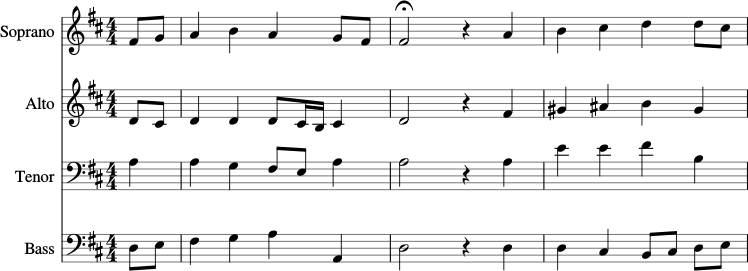
\includegraphics[width=0.8\linewidth]{bwv133-6-original-score-1.png}
    \vspace{1cm}
    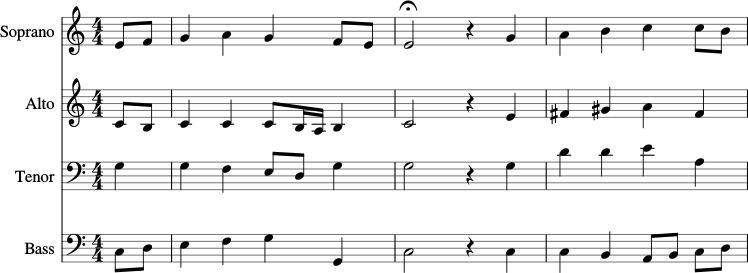
\includegraphics[width=0.8\linewidth]{bwv133-6-preproc-score-1.png}
    \caption{First 4 bars of JCB Chorale BWV 133.6 before (top) and after (bottom) preprocessing. Note
    the transposition down by a semitone to C-major as well as quantization of the
    semiquavers to quavers in Alto bar 2.}
    \label{fig:score-effects-preproc}
\end{figure}

\begin{figure}[htpb]
    \centering
        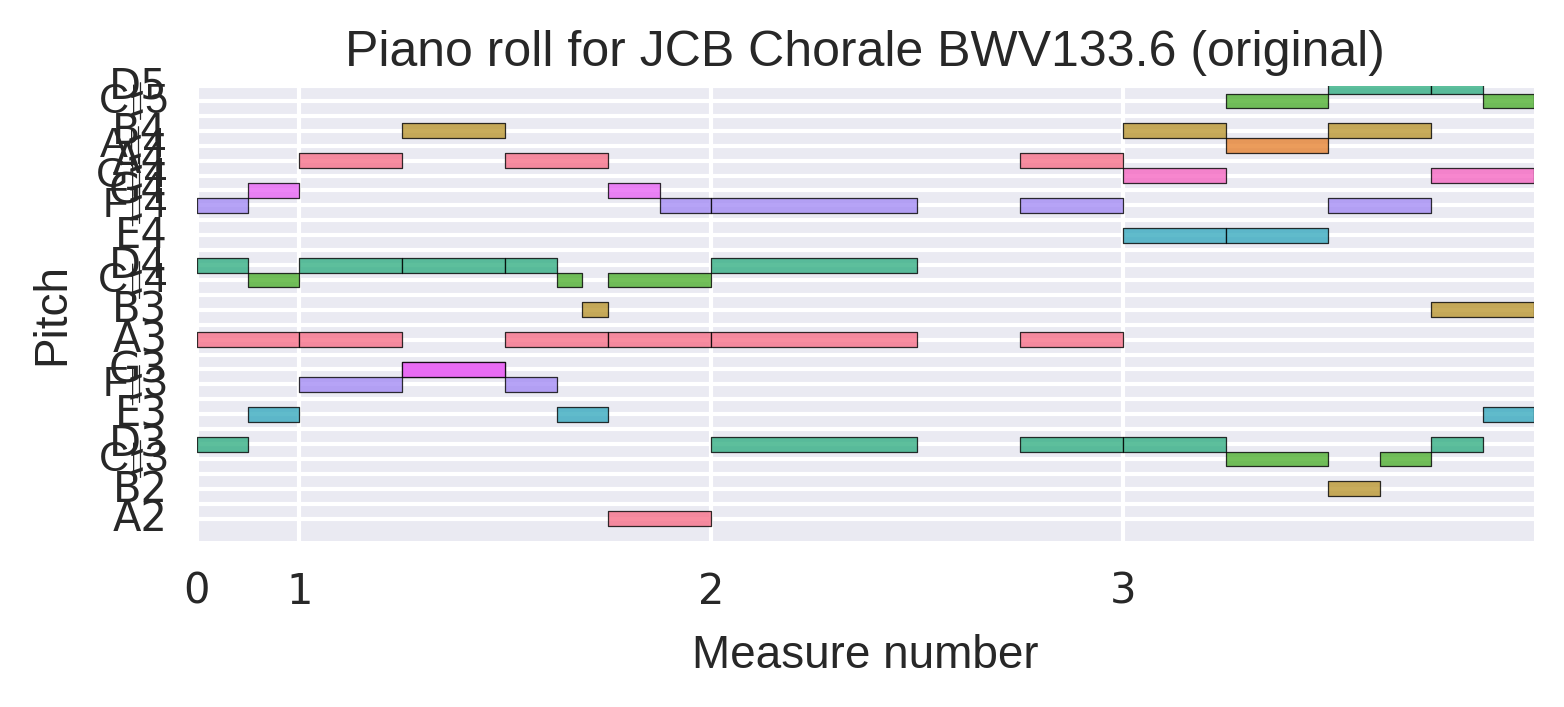
\includegraphics[width=1.0\linewidth]{bwv133-6-original-piano-roll.png}
        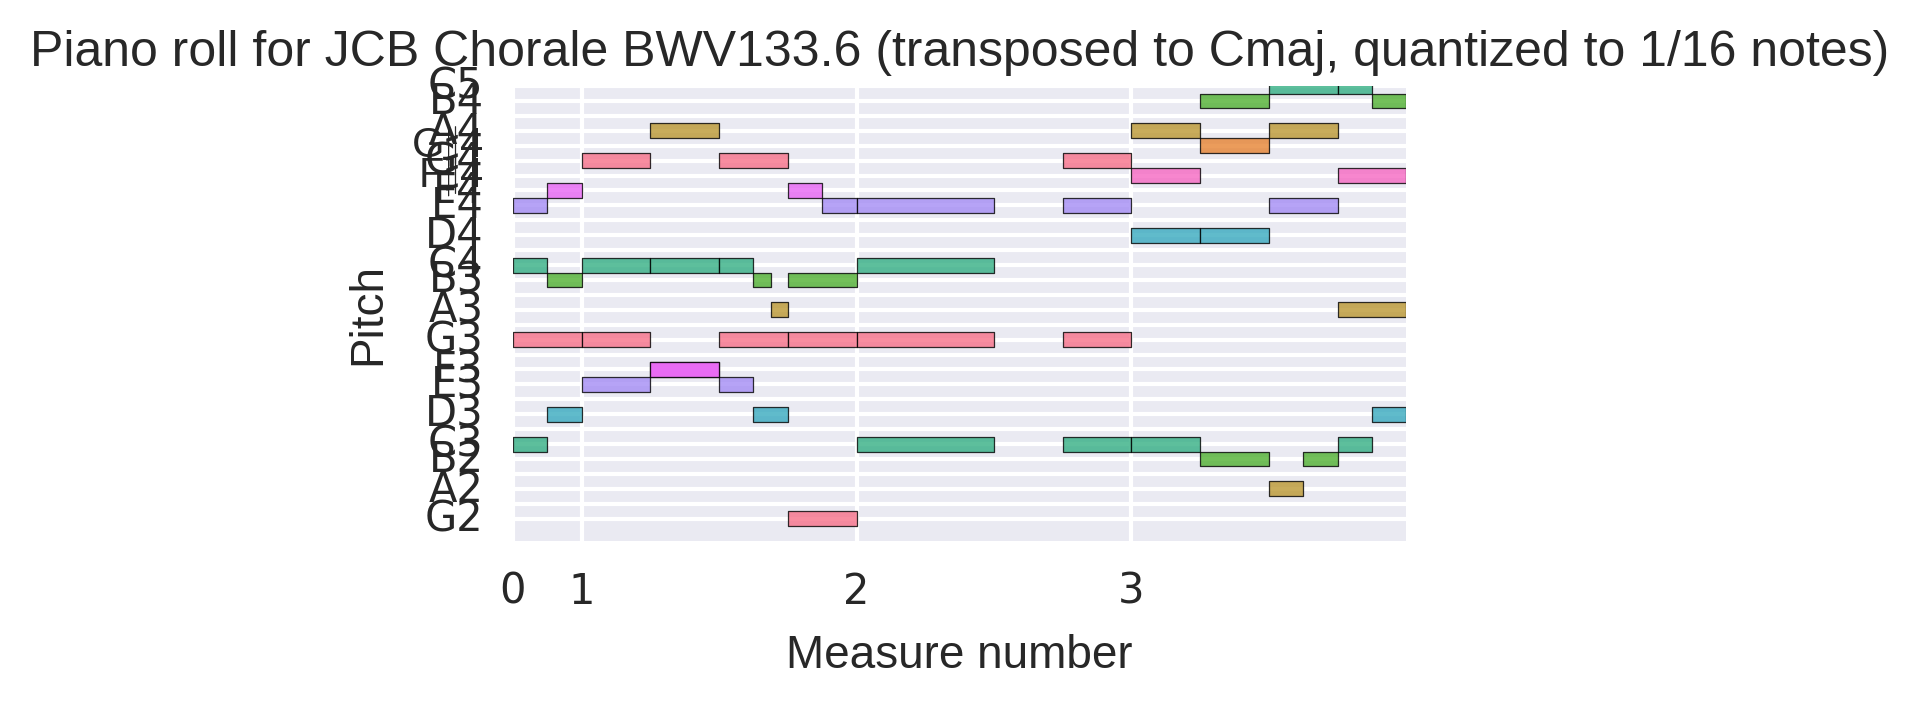
\includegraphics[width=1.0\linewidth]{bwv133-6-preproc-piano-roll.png}
    \caption{Piano roll representation of the same 4 bars from \cref{fig:score-effects-preproc}
    before and after preprocessing.}
    \label{fig:piano-roll-effects-preproc}
\end{figure}

\subsubsection{Corpus level analysis of preprocessing effects}

To assess the effects introduced by key normalization and time quantization,
we analyze corpus level statistics related to pitch and duration.

\cref{fig:pitch-key-standardization} plots a histogram of pitch usage counts
before and after key normalization. Notice that the overall range of pitches
has increased after key normalization. This can be explained by noting that
Bach's chorales were to be performed by vocalists and hence were restricted to
use pitches within human voice ranges regardless of key. After transposition,
this constraint is no longer be satisfied and we see the appearance of
unrealistically low notes (e.g. A1) outside the range of even the lowest voice
types.

\begin{figure}[htpb]
    \centering
    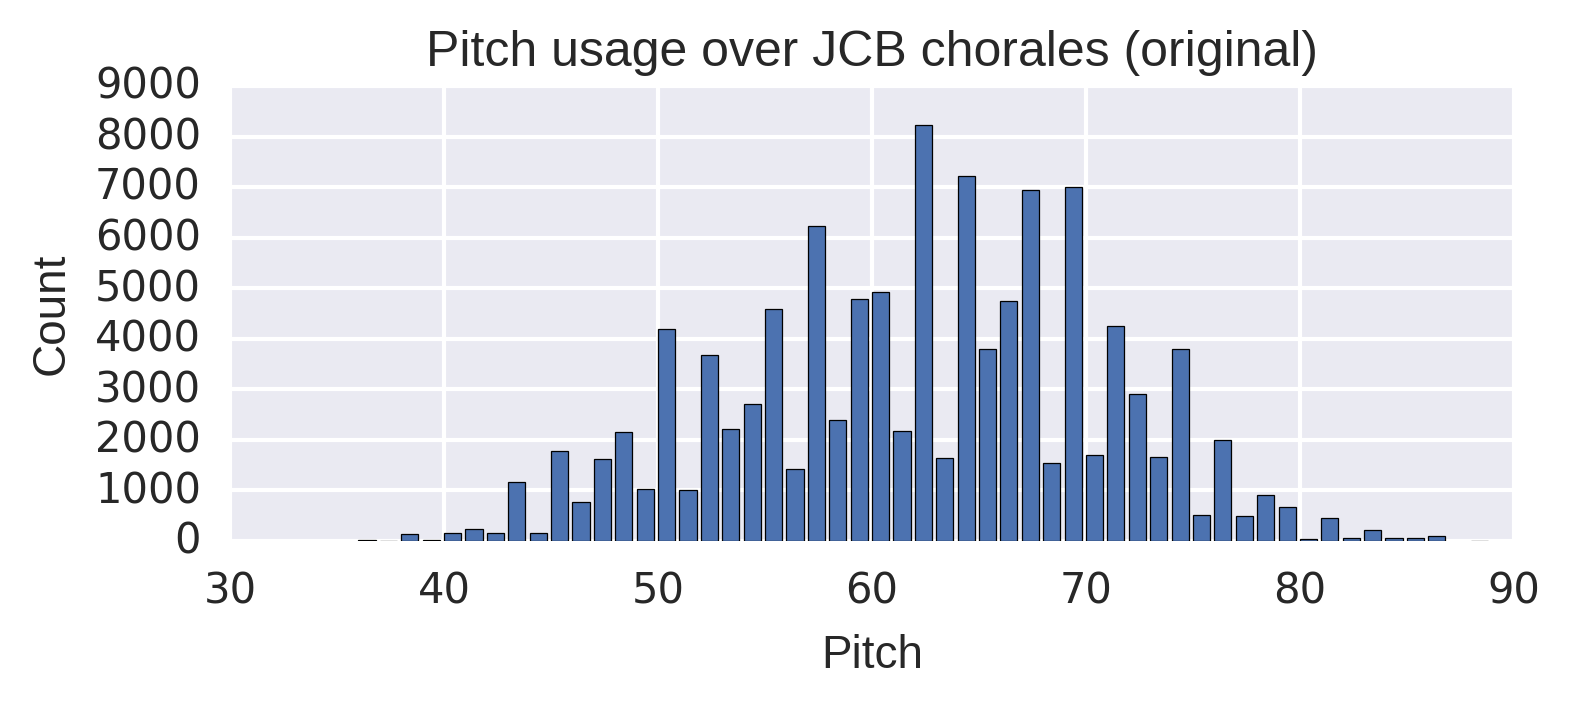
\includegraphics[width=1.0\linewidth]{pitch-usage-original.png}
    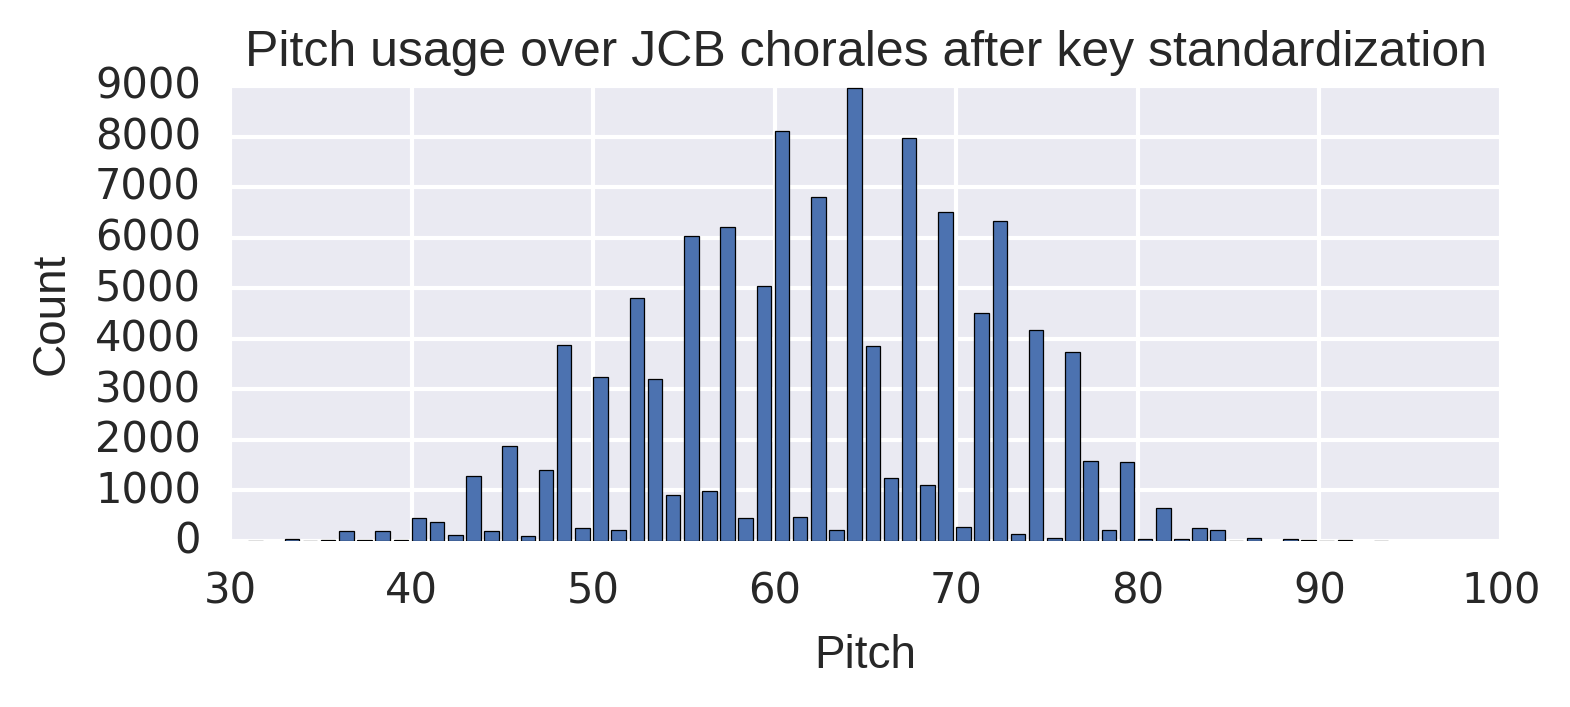
\includegraphics[width=1.0\linewidth]{pitch-usage-preproc.png}
    \caption{Pitches before and after key standardization}
    \label{fig:pitch-key-standardization}
\end{figure}

In \cref{fig:pc-key-standardization}, we visualize histograms of pitch class usages.
As expected, key normalization has increased the usage of pitch classes in the key of
C-major / A-minor (i.e. those which possess no accidentals) and decreased out of key
pitch classes (e.g. C\#, F\#).

\begin{figure}
    \centering
    \begin{subfigure}[b]{0.48\textwidth}
        \centering
        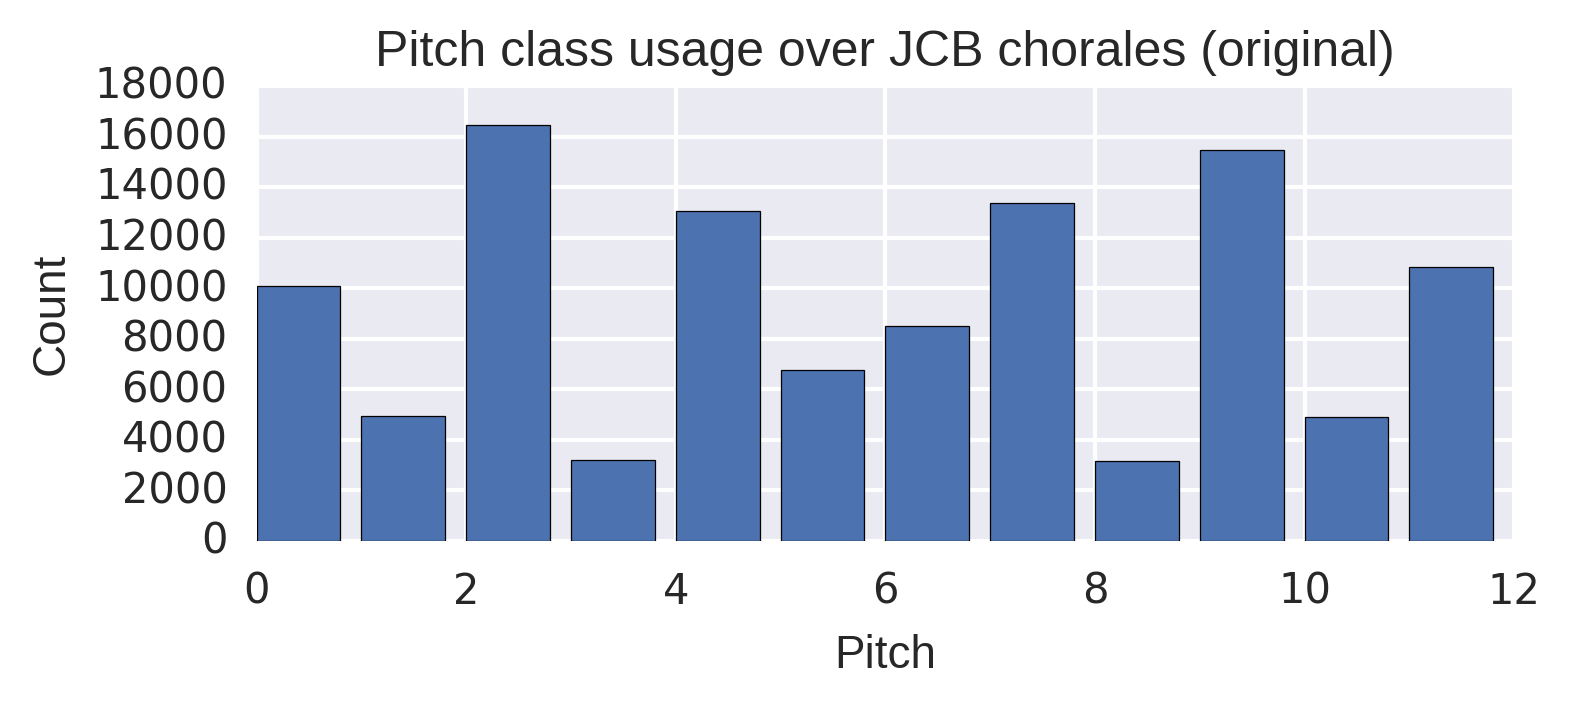
\includegraphics[width=1.0\linewidth]{pitch-class-usage-original.png}
    \end{subfigure}
    \begin{subfigure}[b]{0.48\textwidth}
        \centering
        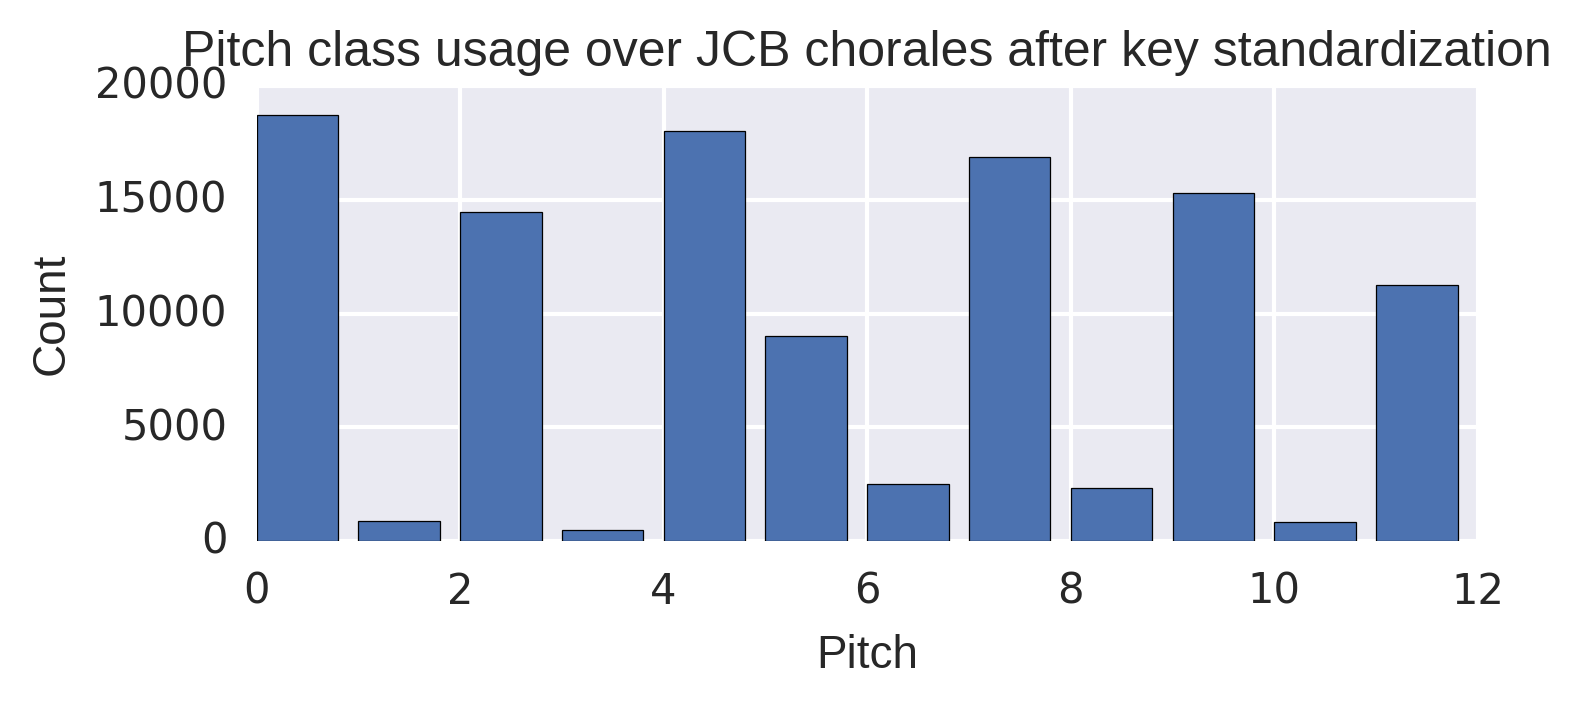
\includegraphics[width=1.0\linewidth]{pitch-class-usage-preproc.png}
    \end{subfigure}
    \caption{Pitch classes before and after key standardization}
    \label{fig:pc-key-standardization}
\end{figure}

We investigate the effects of time quantization in
\cref{fig:note-lengths-time-quantization}, which shows histograms of note
duration usages before and after quantization. \mynote{Update plots... are they affected}.

\begin{figure}[htpb]
    \centering
    \begin{subfigure}[t]{0.48\textwidth}
        \centering
        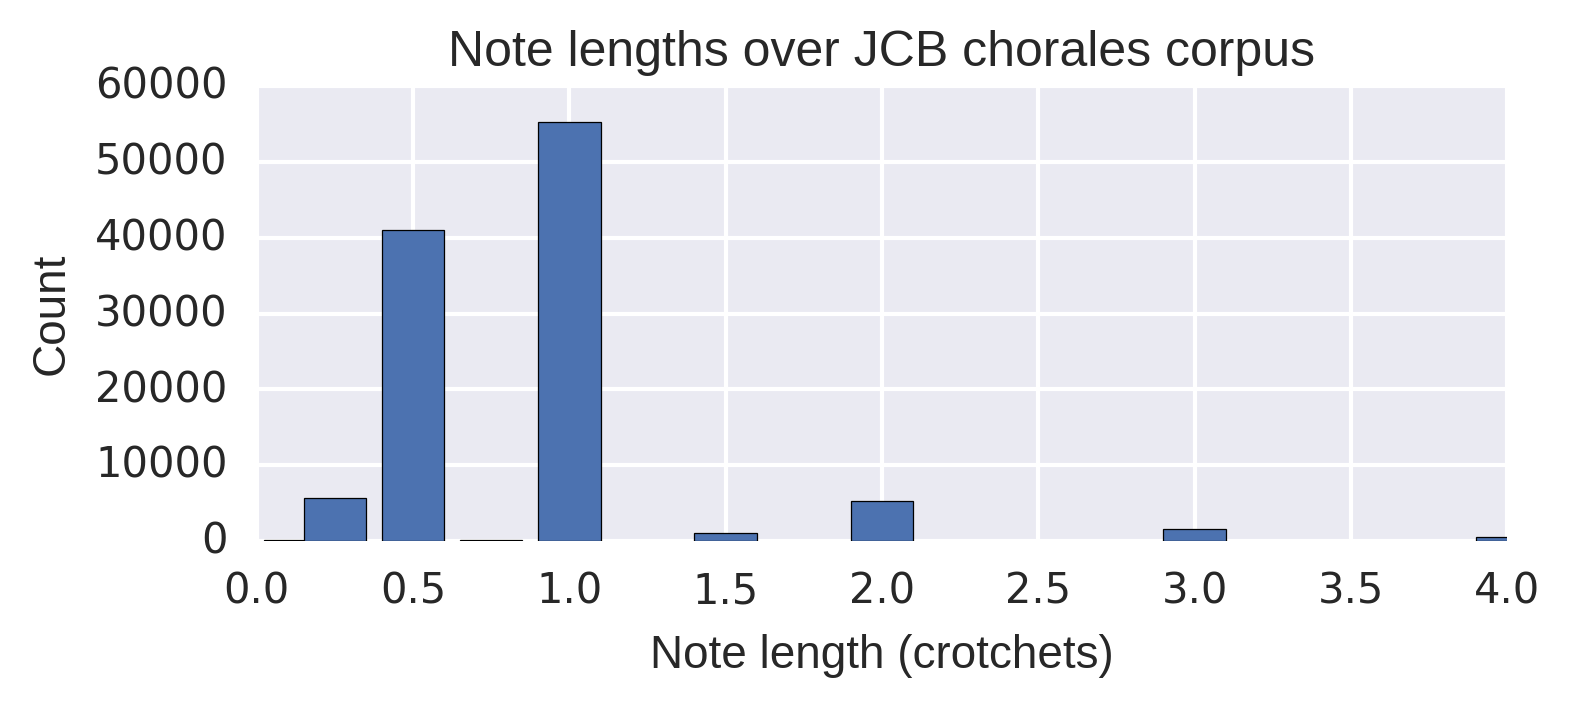
\includegraphics[width=1.0\linewidth]{note-lengths-original.png}
    \end{subfigure}
    \begin{subfigure}[t]{0.48\textwidth}
        \centering
        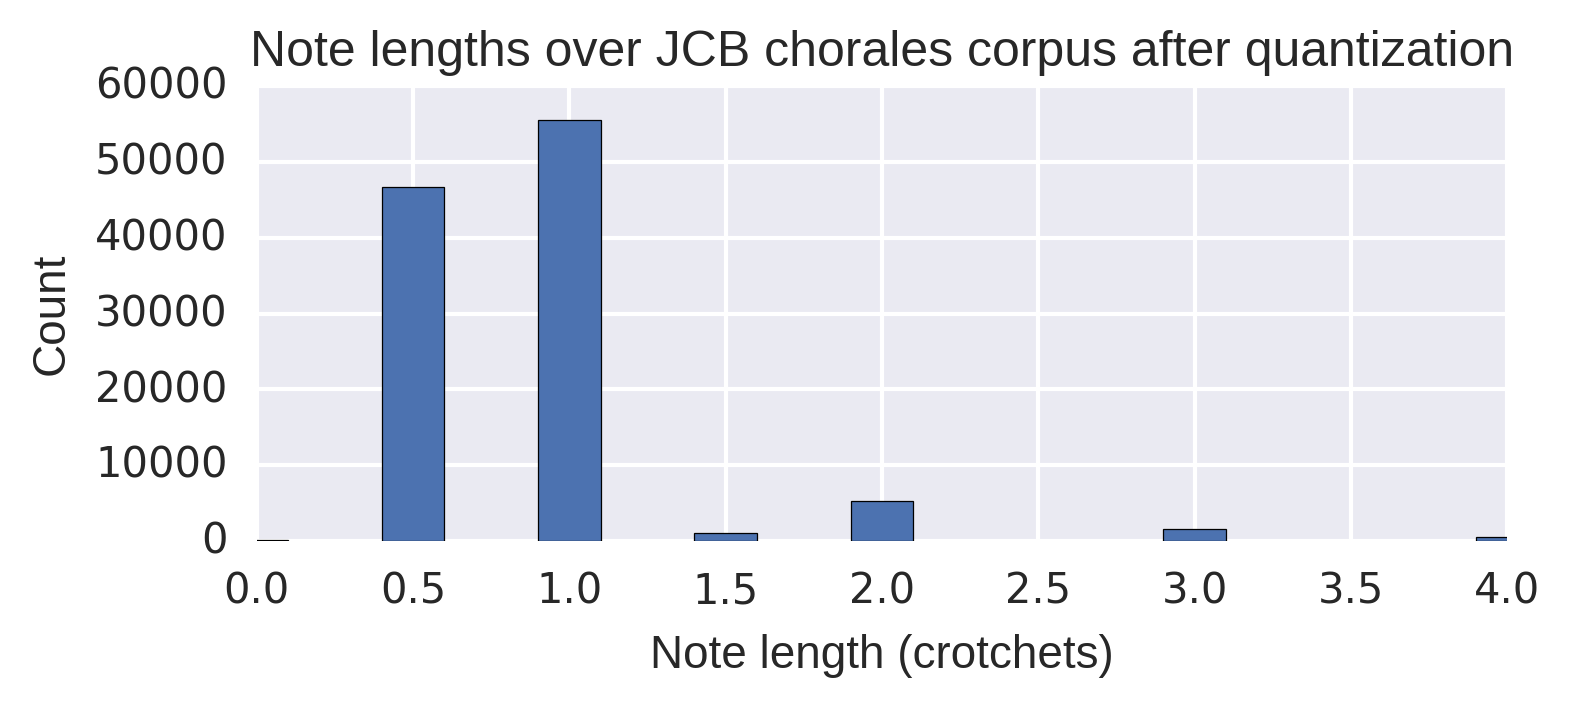
\includegraphics[width=1.0\linewidth]{note-lengths-quantized.png}
    \end{subfigure}
    \caption{Effects of time quantization on note durations}
    \label{fig:note-lengths-time-quantization}
\end{figure}

\begin{figure}[htpb]
    \centering
    \begin{subfigure}[t]{0.48\textwidth}
        \centering
        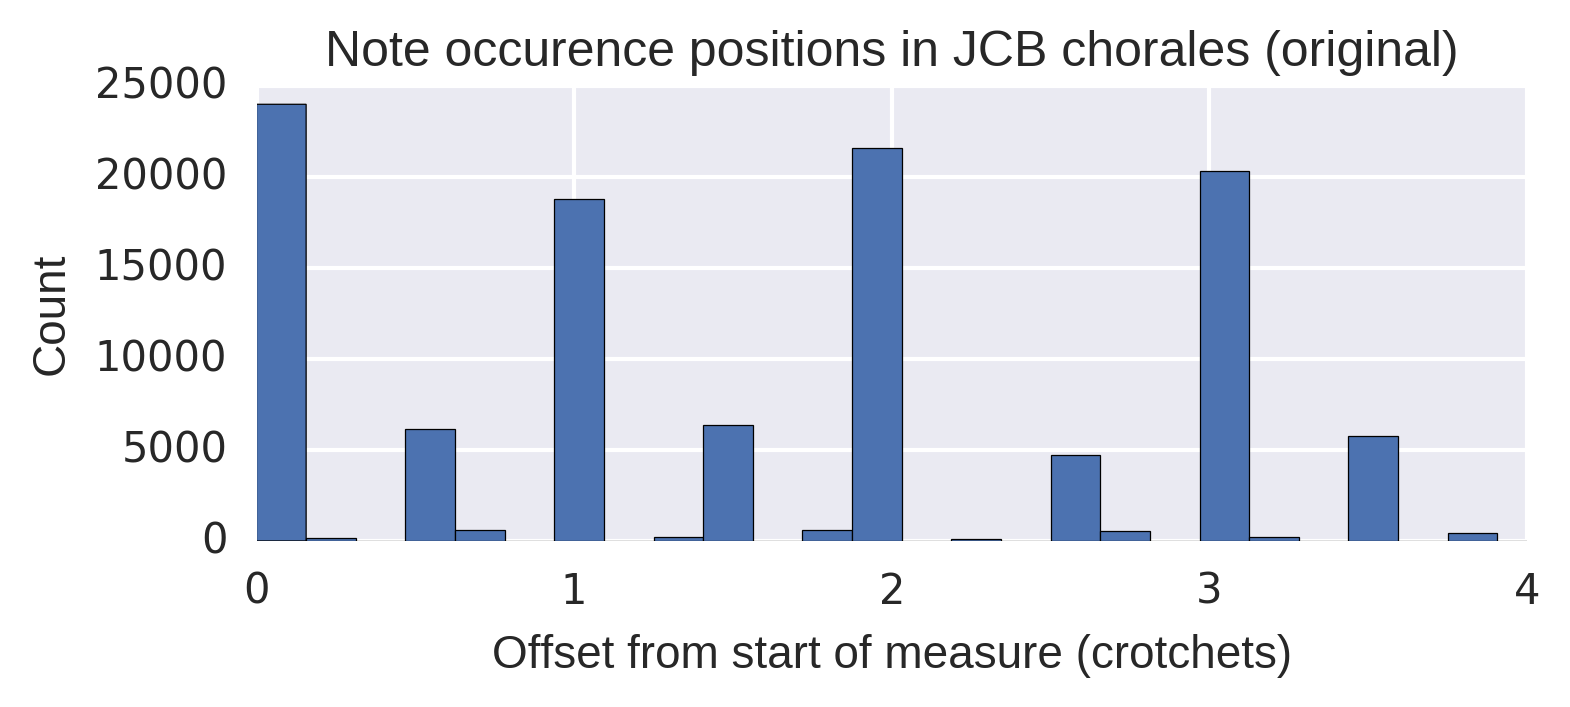
\includegraphics[width=1.0\linewidth]{meter-usage-original.png}
    \end{subfigure}
    ~
    \begin{subfigure}[t]{0.48\textwidth}
        \centering
        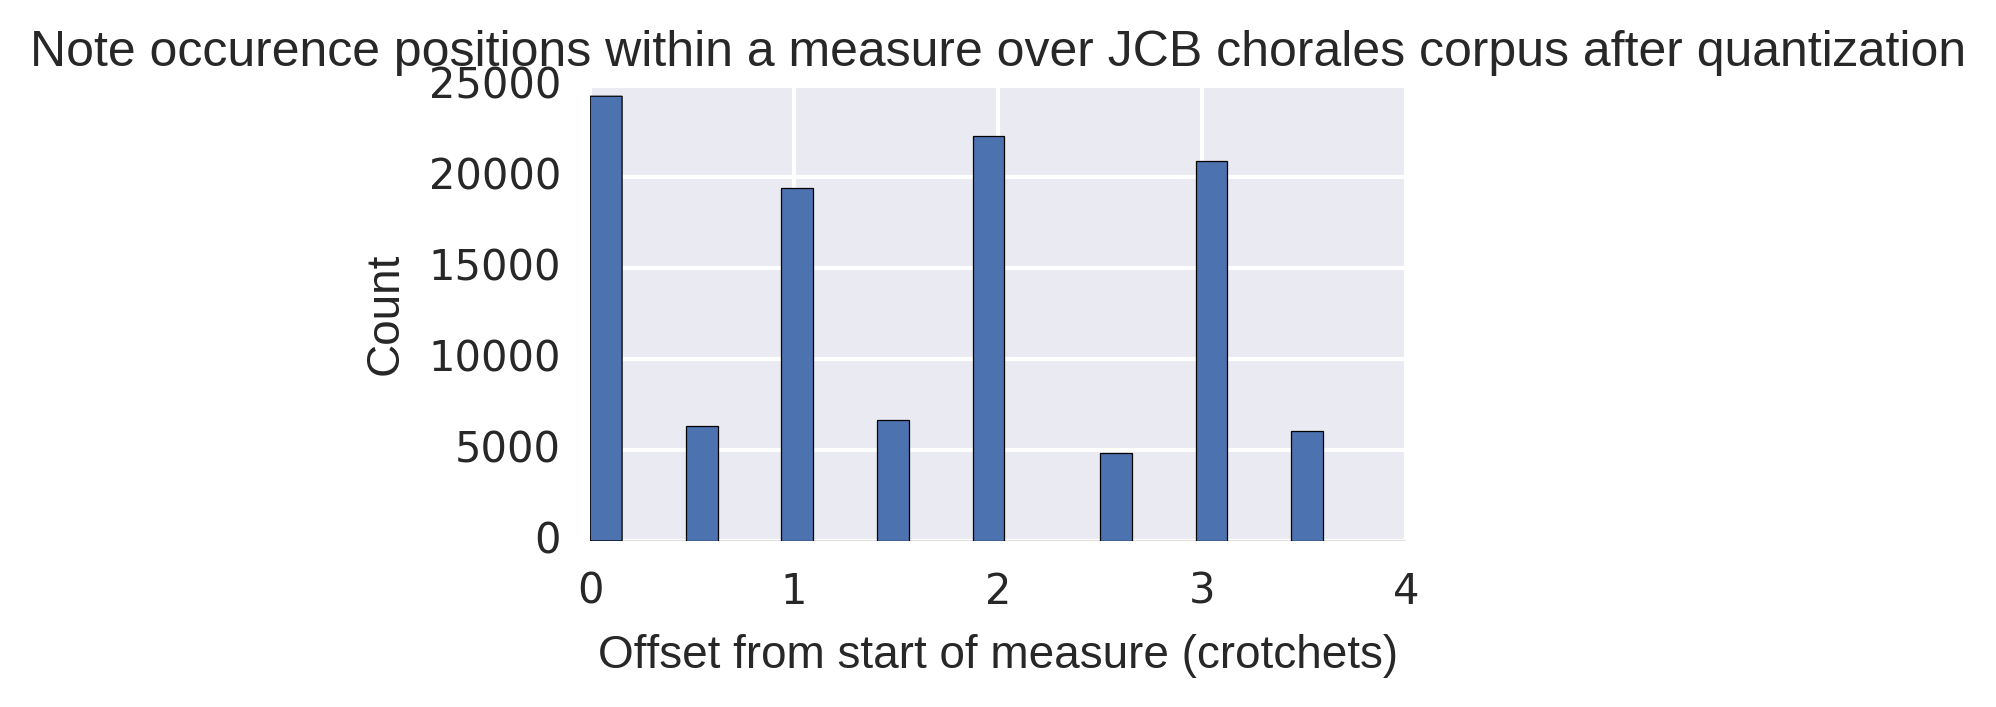
\includegraphics[width=1.0\linewidth]{meter-usage-quantized.png}
    \end{subfigure}
    \caption{Effects of time quantization on meter}
    \label{fig:meter-time-quantization}
\end{figure}

\subsection{Sequential encoding of musical data}

After preprocessing of the scores, our next step is to encode music into a
format amenable for sequential processing. Similar to
\citep{todd1989connectionist}, we represent polyphonic scores using a localist
frame-based representation where time is discretized into constant timestep
\emph{frames}. Frame based processing forces the network to learn the relative
duration of notes, a counting and timing task which \citep{gers2002learning}
demonstred LSTM is capable of. Consecutive frames are separated by a unique
delimiter (``$|||$''' in \mynote{Figure of score encoded in text}).

Each frame consists of a sequence of $\langle \text{Note}, \text{Tie} \rangle$
tuples where $\text{Note} \in \{0,1,\cdots,127\}$ represents the MIDI pitch of
a note and $\text{Tie} \in \{T,F\}$ distinguishes whether a note is tied with a
note at the same pitch from the previous frame or is articulated at the current
timestep. A design decision here is the order in which notes within a frame are
encoded and consequentially processed by a sequential model. Since chorale
music places the melody in the Soprano part, it is reasonable to expect the
Soprano notes to be most significant in determining the other parts. Hence, we
choose to process the Soprano notes first and order notes in descending pitch
within every frame.

The above specification describes our initial encoding. Later in our work
\mynote{reference}, we found that this encoding resulted in unrealistically long
phrase lengths. Including fermatas (represented by ``(.)'' in \mynote{Figure of
encoded score}, which Bach used to denote ends of phrases, solves this problem.

Finally, for each score a unique start symbol (``START'' in \mynote{Figure}) and
end symbol (``END'' in \mynote{Figure}) are appended to the beginning and end
repsectively. This causes the model to learn to initialize itself when given
the start symbol and allows us to determine when a composition generated by the
model has concluded.

Observe that our encoding is sparse: unarticulated notes are not encoded. It is
also variable length as anywhere from zero to four (in the case of chorales,
more for arbitrary polyphonic scores) notes. Finally, the explicit
representation of tied notes vs articulated notes solves the problem plaguing
\citep{Eck2002}\citep{eck2008learning} \citep{Liu2014} \citep{Brien2016} where
multiple articulations at the same pitch are indistinguishable from a single
note with the same duration.

Additionally, notice that our encoding avoids hand-engineered features such as
pitch representations which are psychochologically-based \citep{mozer1994neural}
or harmonically-based \citep{franklin2004recurrent}
\citep{laden1989representation}. This is intentional and is motivated by
numerous reports \citep{bengio2009learning}\citep{Bengio2011} suggesting that
that a key ingredient in deep learning's success is its ability to learn good
features from raw data.

\section{Design and validation of a generative model for music}

In this section, we describe the design and validation process leading to our
generative model. Unlike many prior models for music data, we intentially avoid
injection of domain-specific knowledge into our model architectures such as
distinguishing between chords versus notes
\citep{hild1991harmonet}\citep{mozer1994neural} \citep{Eck2002} and explicitly
modelling of meter \citep{eck2008learning} or motifs \citep{feulner1994melonet}.
Through this fundamental connectionist approach, we aim to minimize biases
introduced by prior assumptions and force the model itself to learn musical
structure from data.

\subsection{Training and evaluation criteria}

Following \citep{mozer1994neural}, we will train the model to predict a distribution
distribution over all possible tokens next $\x_{t+1}$ given the current token
$\x_{t}$ and the previous hidden state $\h_{t-1}$. This is equivalent to
setting the target sequence to be the input sequence delayed by one timestep:
$\y_{1:T-1} = \x_{2:T}$ and $\y_T = \text{STOP}$. \mynote{Diagram for sequential prediction}.
\mynote{Note similarity with language modeling}.

For training criteria, we use the cross-entropy between the predicted
distributions $P(\y_t | \h_t, \x_t)$ and the actual target distribution
$\delta_{\y_t}$.

Note that our training criteria as written in \mynote{reference} uses the actual
next token $\x_{t+1}$ as the recurrent input, even if the most likely
prediction $\argmax P(\x_{t+1} | \h_t, \x_t)$ differs. This is is referred to
as \emph{teacher forcing}\citep{williams1989learning} and is motivated by the
observation that model predictions may not yet be correct during the early
iterations of training. However, at inference the token generated from
$P(\x_{t+1} | \h_t, \x_t)$ is reused as the previous input, creating a
discrepancy between training and inference. Scheduled sampling
\citep{bengio2015scheduled} is a recently proposed alternative training method
for resolving this discrepancy and may help the model better learn to predict
using generated symbols rather than relying on ground truth to be always
provided as input.

\subsection{Comparing memory cells for music data}

Using theanets

One-hot encoding, 64 dimensional vector embedding, RNN layer, fully connected layer, softmax.

\cref{fig:theanets-architecture} compares various RNN architecture performance
through training a RNN with \texttt{num\_layers=1}, \texttt{rnn\_size=130},
\texttt{wordvec=64}.

90/10 train/test split.

\begin{figure}[htpb]
    \centering
    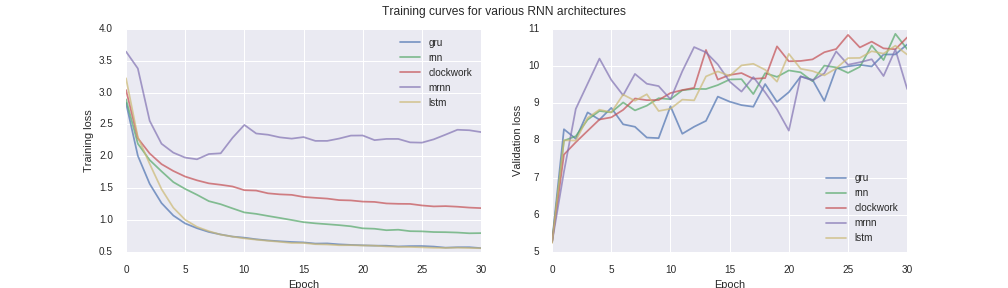
\includegraphics[width=\linewidth]{theanets-architecture.png}
    \caption{theanets-architecture}
    \label{fig:theanets-architecture}
\end{figure}

The LSTM and GRU architectures achieve the lowest training errors, consistent with expectations
since these architectures have the most parameters.
All yielded comparable validation loss which increased over time, motivating regularization.

LSTMs and GRUs trained much faster and achieved lower training loss, suggesting higher capacity.
\citep{Nayebi2015} reports that LSTMs outperform GRUs in music applications, motivating
our final choice for GRUs.

\subsection{Optimizing the LSTM architecture}

Switched to torch-rnn. \mynote{Discrepancy between above architectures and below losses because
  we are perturbing about best model}

We construct multi-layer LSTM models with \texttt{num\_layers} number of
layers, each containing \texttt{rnn\_size} hidden units. The inputs $x_t$ are
one-hot-encoded before being passed through a \texttt{wordvec}-dimensional
vector-space embedding layer, which compresses the dimensionality down from
$|V| \approx 140$ to $\texttt{wordvec}$ dimensions. Dropout layers were added
between LSTM connections in both depth and time dimensions all with dropout
probability $\texttt{dropout} \in [0,1]$.

We build our models using the \texttt{torch7} framework and
an optimized implementation of LSTMs provided by \texttt{torch-rnn} \mynote{citep}.

Models were trained using RMSProp \mynote{citep} with batch normalization \mynote{citep}
and an initial learning rate of $2 \times 10^{-3}$ decayed by $0.5$ every $5$
epochs. The back-propogation through time gradients were clipped
at $t$ \mynote{citep Mikolov} and truncated after \texttt{seq\_length} time steps.
We use a mini-batch size of $50$.

\subsubsection{Overall best model}

We identified our best model to be \mynote{what is it?}.

\begin{figure}[htpb]
  \centering
  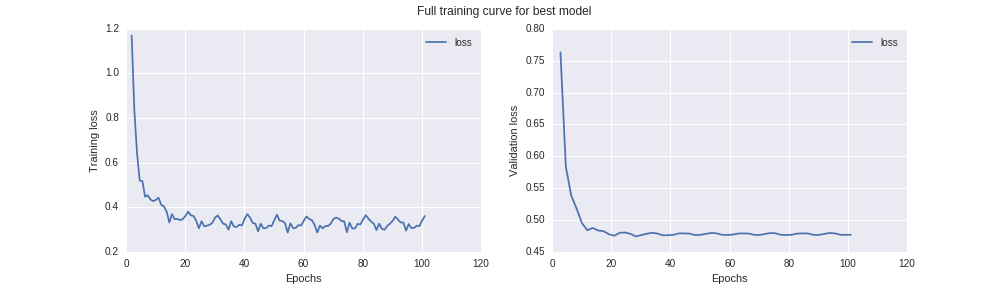
\includegraphics[width=1.0\linewidth]{torch-rnn-best-model-trace.png}
  \caption{torch-rnn-best-model-Trace}
  \label{fig:torch-rnn-best-model-trace}
\end{figure}

In the following sections, we investigate pertubations about this model and the
effects of various hyperparameters. A complete listing of results are available
in
\cref{tab:torch-rnn-config-perfs}.
\begin{table}[htpb]
    \centering
    \caption{Performance of various LSTM configurations}
    \label{tab:torch-rnn-config-perfs}
    \begin{longtable}{rrrrrr}
\toprule
 num\_layers &  rnn\_size &  seq\_length &  wordvec &  train\_metric &  val\_metric \\
\midrule
\endhead
\midrule
\multicolumn{3}{r}{{Continued on next page}} \\
\midrule
\endfoot

\bottomrule
\endlastfoot
        3.0 &     256.0 &       128.0 &     32.0 &      0.323781 &    0.477027 \\
        2.0 &     256.0 &       128.0 &     32.0 &      0.323668 &    0.479322 \\
        2.0 &     256.0 &       128.0 &     64.0 &      0.303158 &    0.482216 \\
        3.0 &     256.0 &       256.0 &     64.0 &      0.320361 &    0.484231 \\
        3.0 &     256.0 &       128.0 &     32.0 &      0.383811 &    0.484667 \\
        3.0 &     256.0 &       128.0 &     16.0 &      0.342955 &    0.484791 \\
        2.0 &     256.0 &       256.0 &     64.0 &      0.373641 &    0.485353 \\
        3.0 &     256.0 &       128.0 &     64.0 &      0.305290 &    0.486244 \\
        2.0 &     256.0 &       128.0 &     32.0 &      0.275125 &    0.486305 \\
        2.0 &     256.0 &       256.0 &     32.0 &      0.352257 &    0.486755 \\
        4.0 &     256.0 &       128.0 &     32.0 &      0.333133 &    0.487135 \\
        2.0 &     256.0 &       256.0 &     32.0 &      0.307188 &    0.487868 \\
        2.0 &     256.0 &       256.0 &     32.0 &      0.400955 &    0.489320 \\
        3.0 &     256.0 &       256.0 &     64.0 &      0.381868 &    0.489810 \\
        2.0 &     256.0 &       256.0 &     64.0 &      0.333356 &    0.491396 \\
        2.0 &     256.0 &       256.0 &     64.0 &      0.284248 &    0.491593 \\
        3.0 &     128.0 &       128.0 &     32.0 &      0.365171 &    0.492478 \\
        3.0 &     256.0 &       128.0 &     32.0 &      0.264723 &    0.492849 \\
        3.0 &     384.0 &       128.0 &     32.0 &      0.228556 &    0.495991 \\
        3.0 &     256.0 &       128.0 &     64.0 &      0.248987 &    0.496190 \\
        3.0 &     256.0 &       128.0 &     32.0 &      0.445840 &    0.498205 \\
        3.0 &     256.0 &       256.0 &     32.0 &      0.273567 &    0.499422 \\
        2.0 &     256.0 &       128.0 &     64.0 &      0.256022 &    0.500500 \\
        3.0 &     256.0 &       256.0 &     32.0 &      0.338776 &    0.501711 \\
        2.0 &     128.0 &       128.0 &     32.0 &      0.384075 &    0.501840 \\
        3.0 &     128.0 &       128.0 &     64.0 &      0.417780 &    0.501919 \\
        2.0 &     256.0 &       128.0 &     32.0 &      0.219939 &    0.502503 \\
        3.0 &     128.0 &       128.0 &     64.0 &      0.361381 &    0.503206 \\
        3.0 &     128.0 &       128.0 &     32.0 &      0.431771 &    0.503590 \\
        3.0 &     256.0 &        64.0 &     64.0 &      0.263001 &    0.503945 \\
        3.0 &     256.0 &       384.0 &     64.0 &      0.419091 &    0.504249 \\
        3.0 &     256.0 &       256.0 &     32.0 &      0.393463 &    0.506486 \\
        2.0 &     128.0 &       128.0 &     64.0 &      0.364640 &    0.506923 \\
        2.0 &     128.0 &       128.0 &     64.0 &      0.422178 &    0.507268 \\
        3.0 &     256.0 &       256.0 &     64.0 &      0.261563 &    0.507479 \\
        3.0 &     256.0 &        64.0 &     32.0 &      0.278916 &    0.507673 \\
        2.0 &     128.0 &       128.0 &     32.0 &      0.434552 &    0.508460 \\
        3.0 &     256.0 &       384.0 &     32.0 &      0.439684 &    0.514804 \\
        1.0 &     256.0 &       128.0 &     64.0 &      0.334873 &    0.517134 \\
        2.0 &     128.0 &       128.0 &     64.0 &      0.465061 &    0.520224 \\
        2.0 &     256.0 &       128.0 &     64.0 &      0.195905 &    0.521330 \\
        1.0 &     256.0 &       256.0 &     64.0 &      0.368281 &    0.522424 \\
        2.0 &     128.0 &       128.0 &     32.0 &      0.485346 &    0.522955 \\
        2.0 &     128.0 &       256.0 &     64.0 &      0.378280 &    0.525397 \\
        3.0 &     512.0 &       128.0 &     32.0 &      0.168366 &    0.525644 \\
        1.0 &     256.0 &       256.0 &     64.0 &      0.417803 &    0.525980 \\
        3.0 &     128.0 &       128.0 &     64.0 &      0.480340 &    0.526121 \\
        3.0 &     128.0 &       128.0 &     32.0 &      0.491876 &    0.527008 \\
        3.0 &     256.0 &       128.0 &     32.0 &      0.194120 &    0.528000 \\
        2.0 &     128.0 &       128.0 &     64.0 &      0.296537 &    0.528261 \\
        2.0 &     128.0 &       128.0 &     32.0 &      0.316390 &    0.529308 \\
        3.0 &     128.0 &       256.0 &     64.0 &      0.435649 &    0.529458 \\
        1.0 &     256.0 &       128.0 &     32.0 &      0.375717 &    0.529638 \\
        2.0 &     128.0 &       256.0 &     64.0 &      0.440450 &    0.529948 \\
        1.0 &     256.0 &       256.0 &     64.0 &      0.389651 &    0.531063 \\
        2.0 &     128.0 &       256.0 &    128.0 &      0.362561 &    0.533559 \\
        2.0 &     128.0 &       256.0 &     32.0 &      0.398919 &    0.533672 \\
        3.0 &     128.0 &       256.0 &     32.0 &      0.452009 &    0.536955 \\
        1.0 &     256.0 &       128.0 &     32.0 &      0.346140 &    0.538510 \\
        2.0 &     128.0 &       128.0 &    128.0 &      0.273516 &    0.539359 \\
        1.0 &     256.0 &       128.0 &     64.0 &      0.310597 &    0.539599 \\
        3.0 &     128.0 &       128.0 &     32.0 &      0.265842 &    0.539827 \\
        1.0 &     256.0 &       128.0 &     64.0 &      0.274568 &    0.541263 \\
        3.0 &     128.0 &       256.0 &     64.0 &      0.500697 &    0.544048 \\
        1.0 &     256.0 &       128.0 &     32.0 &      0.316189 &    0.545363 \\
        1.0 &     256.0 &       128.0 &     32.0 &      0.285714 &    0.546995 \\
        3.0 &     128.0 &       128.0 &     64.0 &      0.247192 &    0.549826 \\
        1.0 &     128.0 &       128.0 &     64.0 &      0.458142 &    0.550102 \\
        1.0 &     128.0 &       128.0 &    128.0 &      0.360038 &    0.550509 \\
        2.0 &     128.0 &       256.0 &     32.0 &      0.465110 &    0.550995 \\
        1.0 &     256.0 &       256.0 &     32.0 &      0.444180 &    0.551894 \\
        3.0 &     256.0 &       128.0 &     64.0 &      0.184959 &    0.552200 \\
        2.0 &     128.0 &       256.0 &     64.0 &      0.490587 &    0.552217 \\
        2.0 &     128.0 &       256.0 &     32.0 &      0.514900 &    0.553092 \\
        1.0 &     128.0 &       128.0 &     64.0 &      0.487574 &    0.553498 \\
        1.0 &     256.0 &       256.0 &     32.0 &      0.471938 &    0.553586 \\
        1.0 &     128.0 &       128.0 &     64.0 &      0.384282 &    0.554990 \\
        1.0 &     128.0 &       128.0 &     64.0 &      0.425469 &    0.555312 \\
        1.0 &     256.0 &       256.0 &     32.0 &      0.411686 &    0.555955 \\
        1.0 &     256.0 &       128.0 &     64.0 &      0.238860 &    0.556672 \\
        3.0 &      64.0 &       128.0 &     64.0 &      0.420250 &    0.559336 \\
        3.0 &      64.0 &        64.0 &    128.0 &      0.345705 &    0.559549 \\
        3.0 &     128.0 &       128.0 &    128.0 &      0.238071 &    0.562603 \\
        2.0 &     256.0 &       128.0 &     32.0 &      0.143647 &    0.563866 \\
        1.0 &     128.0 &       128.0 &     32.0 &      0.489160 &    0.564304 \\
        3.0 &     128.0 &       256.0 &     32.0 &      0.521478 &    0.566153 \\
        2.0 &     128.0 &       128.0 &     64.0 &      0.584950 &    0.567093 \\
        2.0 &      64.0 &       128.0 &     64.0 &      0.443393 &    0.567754 \\
        2.0 &     128.0 &       256.0 &     64.0 &      0.549169 &    0.568419 \\
        1.0 &     128.0 &        64.0 &     32.0 &      0.359041 &    0.569011 \\
        3.0 &     128.0 &       256.0 &     64.0 &      0.573862 &    0.570873 \\
        1.0 &     128.0 &       128.0 &     32.0 &      0.525982 &    0.571859 \\
        3.0 &      64.0 &       128.0 &    128.0 &      0.408074 &    0.572306 \\
        1.0 &     128.0 &       128.0 &     32.0 &      0.467434 &    0.572480 \\
        1.0 &     128.0 &       128.0 &     32.0 &      0.417764 &    0.573797 \\
        2.0 &      64.0 &        64.0 &     32.0 &      0.413944 &    0.573993 \\
        3.0 &      64.0 &        64.0 &     64.0 &      0.355615 &    0.574236 \\
        1.0 &     256.0 &       128.0 &    128.0 &      0.204964 &    0.574585 \\
        1.0 &     128.0 &        64.0 &     64.0 &      0.328927 &    0.575464 \\
        2.0 &      64.0 &        64.0 &     64.0 &      0.390597 &    0.575592 \\
        2.0 &      64.0 &       128.0 &    128.0 &      0.424735 &    0.575868 \\
        2.0 &      64.0 &        32.0 &     32.0 &      0.399389 &    0.577974 \\
        2.0 &      64.0 &        64.0 &    128.0 &      0.372478 &    0.578856 \\
        2.0 &     128.0 &        64.0 &     32.0 &      0.240288 &    0.580802 \\
        3.0 &      64.0 &        64.0 &     32.0 &      0.375478 &    0.582072 \\
        1.0 &     128.0 &        64.0 &    128.0 &      0.304245 &    0.582897 \\
        3.0 &      64.0 &       128.0 &     32.0 &      0.430421 &    0.582991 \\
        3.0 &     128.0 &       256.0 &     32.0 &      0.590133 &    0.585245 \\
        3.0 &      64.0 &        32.0 &     32.0 &      0.348150 &    0.585800 \\
        2.0 &      64.0 &        32.0 &     64.0 &      0.387047 &    0.589173 \\
        1.0 &     128.0 &       256.0 &     64.0 &      0.501138 &    0.593823 \\
        3.0 &      64.0 &        32.0 &    128.0 &      0.339394 &    0.594401 \\
        1.0 &     128.0 &        32.0 &     32.0 &      0.348193 &    0.595001 \\
        2.0 &      64.0 &       128.0 &     32.0 &      0.470837 &    0.597005 \\
        3.0 &      64.0 &        32.0 &     64.0 &      0.344404 &    0.597406 \\
        2.0 &     128.0 &        64.0 &     64.0 &      0.224014 &    0.597418 \\
        1.0 &      64.0 &        32.0 &     64.0 &      0.462827 &    0.597437 \\
        1.0 &      64.0 &        32.0 &     32.0 &      0.500014 &    0.598521 \\
        2.0 &      64.0 &        32.0 &    128.0 &      0.376624 &    0.600570 \\
        1.0 &      64.0 &        32.0 &    128.0 &      0.453646 &    0.604043 \\
        1.0 &     128.0 &       256.0 &     64.0 &      0.539087 &    0.604710 \\
        2.0 &     256.0 &       128.0 &     64.0 &      0.122328 &    0.606237 \\
        1.0 &      64.0 &       128.0 &    128.0 &      0.489255 &    0.607122 \\
        1.0 &     128.0 &        32.0 &     64.0 &      0.319029 &    0.609441 \\
        1.0 &     128.0 &       256.0 &     64.0 &      0.566182 &    0.610409 \\
        1.0 &     128.0 &        32.0 &    128.0 &      0.294204 &    0.613838 \\
        1.0 &      64.0 &        64.0 &    128.0 &      0.436633 &    0.615036 \\
        1.0 &      64.0 &        64.0 &     64.0 &      0.461935 &    0.616265 \\
        2.0 &     128.0 &        64.0 &    128.0 &      0.206896 &    0.620845 \\
        1.0 &     128.0 &       256.0 &     32.0 &      0.550056 &    0.627652 \\
        2.0 &     256.0 &       128.0 &    128.0 &      0.106181 &    0.631364 \\
        3.0 &     128.0 &        64.0 &     32.0 &      0.185779 &    0.633145 \\
        1.0 &     128.0 &       256.0 &     32.0 &      0.591930 &    0.638022 \\
        1.0 &     256.0 &        64.0 &     32.0 &      0.200897 &    0.640652 \\
        1.0 &      64.0 &        64.0 &     32.0 &      0.487779 &    0.643943 \\
        1.0 &     128.0 &       256.0 &     32.0 &      0.621720 &    0.647467 \\
        2.0 &     128.0 &        32.0 &     32.0 &      0.209044 &    0.647553 \\
        3.0 &     256.0 &       128.0 &     32.0 &      0.100153 &    0.650138 \\
        1.0 &      64.0 &       128.0 &     64.0 &      0.515733 &    0.653191 \\
        1.0 &     256.0 &        64.0 &     64.0 &      0.171567 &    0.657626 \\
        3.0 &     256.0 &       128.0 &     64.0 &      0.087426 &    0.660995 \\
        3.0 &     128.0 &        64.0 &    128.0 &      0.169560 &    0.663409 \\
        3.0 &     128.0 &        64.0 &     64.0 &      0.172871 &    0.670402 \\
        1.0 &      64.0 &       128.0 &     32.0 &      0.561724 &    0.670482 \\
        1.0 &     256.0 &        64.0 &    128.0 &      0.149129 &    0.672432 \\
        2.0 &     128.0 &        32.0 &     64.0 &      0.193615 &    0.688310 \\
        2.0 &     128.0 &       128.0 &     64.0 &      0.802259 &    0.696580 \\
        2.0 &     128.0 &       256.0 &     32.0 &      0.907374 &    0.701893 \\
        3.0 &     256.0 &       128.0 &    128.0 &      0.076598 &    0.711632 \\
        2.0 &     256.0 &        64.0 &     32.0 &      0.081134 &    0.716840 \\
        2.0 &     128.0 &        32.0 &    128.0 &      0.173684 &    0.727354 \\
        2.0 &     256.0 &        64.0 &     64.0 &      0.073675 &    0.742250 \\
        1.0 &     256.0 &        32.0 &     32.0 &      0.161496 &    0.743529 \\
        3.0 &     128.0 &        32.0 &     32.0 &      0.146775 &    0.752404 \\
        1.0 &     256.0 &        32.0 &     64.0 &      0.138145 &    0.755407 \\
        1.0 &     256.0 &        32.0 &    128.0 &      0.125931 &    0.757801 \\
        3.0 &     128.0 &        32.0 &     64.0 &      0.134530 &    0.770094 \\
        2.0 &     256.0 &        64.0 &    128.0 &      0.063084 &    0.797383 \\
        3.0 &     128.0 &        32.0 &    128.0 &      0.129410 &    0.801131 \\
        3.0 &     256.0 &        64.0 &     64.0 &      0.048852 &    0.823713 \\
        3.0 &     256.0 &        64.0 &     32.0 &      0.052363 &    0.848516 \\
        2.0 &     256.0 &        32.0 &     32.0 &      0.058634 &    0.874037 \\
        3.0 &     256.0 &        64.0 &    128.0 &      0.044448 &    0.876398 \\
        2.0 &     256.0 &        32.0 &    128.0 &      0.049791 &    0.888397 \\
        2.0 &     256.0 &        32.0 &     64.0 &      0.050012 &    0.898488 \\
        3.0 &     256.0 &        32.0 &     32.0 &      0.037417 &    0.960396 \\
        3.0 &     256.0 &        32.0 &     64.0 &      0.034403 &    0.988554 \\
        3.0 &     256.0 &        32.0 &    128.0 &      0.036275 &    0.990457 \\
\end{longtable}

\end{table}

\subsubsection{Regularization}

The increasing validation error in \cref{fig:theanets-architecture} confirmed
that our models were overfitting and required regularization. \texttt{dropout}

\begin{figure}[htpb]
  \centering
  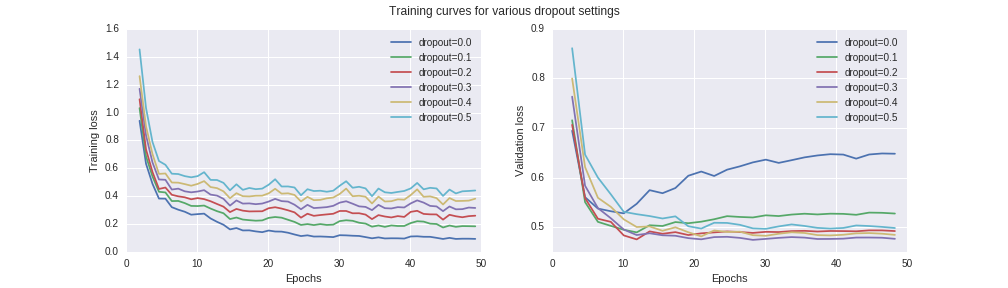
\includegraphics[width=1.0\linewidth]{torch-rnn-dropout.png}
  \caption{torch-rnn-Dropout}
  \label{fig:torch-rnn-dropout}
\end{figure}

\mynote{Batch normalization experiments}

\subsubsection{Network capacity}

\begin{figure}[htpb]
    \centering
    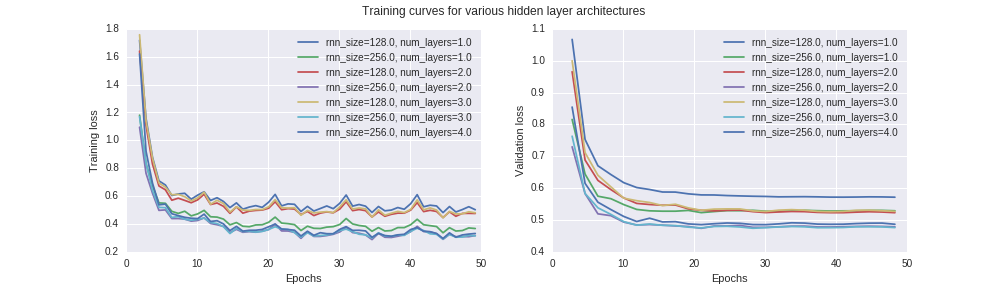
\includegraphics[width=\linewidth]{torch-rnn-network-params.png}
    \caption{torch-rnn-network-params}
    \label{fig:torch-rnn-network-params}
\end{figure}

\begin{figure}[htpb]
  \centering
  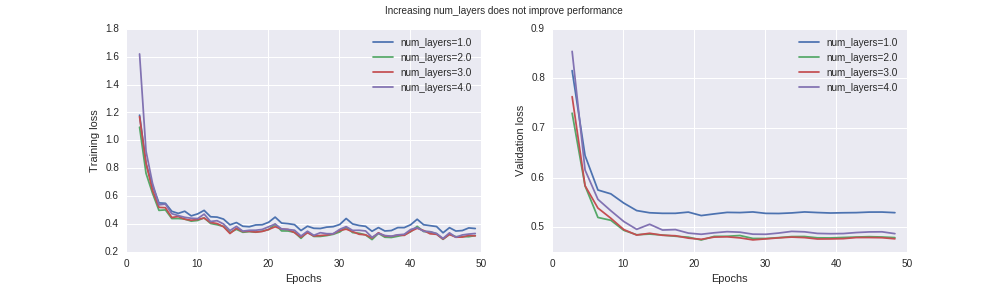
\includegraphics[width=1.0\linewidth]{torch-rnn-network-params-num-layers.png}
  \caption{torch-rnn-network-params-num-Layers}
  \label{fig:torch-rnn-network-params-num-layers}
\end{figure}

\begin{figure}[htpb]
  \centering
  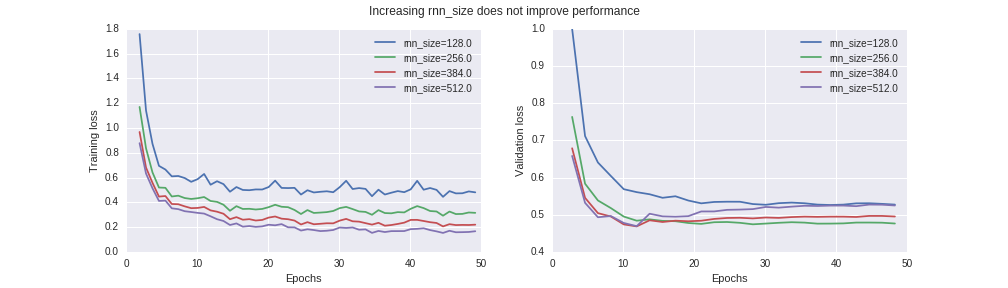
\includegraphics[width=1.0\linewidth]{torch-rnn-network-params-rnn-size.png}
  \caption{torch-rnn-network-params-rnn-size}
  \label{fig:torch-rnn-network-params-rnn-size}
\end{figure}

Sensitivity to network structure: \texttt{num\_layers} and \texttt{rnn\_size}.
\begin{itemize}
    \item Larger \texttt{rnn\_size} leads to higher capacity and lower training loss
        \begin{itemize}
            \item Presents as overfitting on validation, where the lowest capacity
                model \texttt{rnn\_size} appears to be improving in generalization while
                others are flat/increasing
        \end{itemize}
    \item Training curves about the same wrt \texttt{num\_layers}, validation curves have interesting story
        \begin{itemize}
            \item Depth matters: small 64 and 128 hidden unit RNNs saw improvements up to 0.09
            \item Expressivity gained from depth furthers overfitting: 256
                hidden unit RNN has some of the best validation performance at
                depth 1 but is the worst generalizing model for depths 2
                and 3 even though training loss is low
        \end{itemize}
    \item \texttt{rnn\_size=128} undisputably best generalizing, optimized at
        \texttt{num\_layers=2}: will continue with these settings
\end{itemize}

\subsubsection{Network input parameters}

\mynote{Is seq\_length an input parameter, or the BPTT parameters?}

\begin{figure}[htpb]
    \centering
    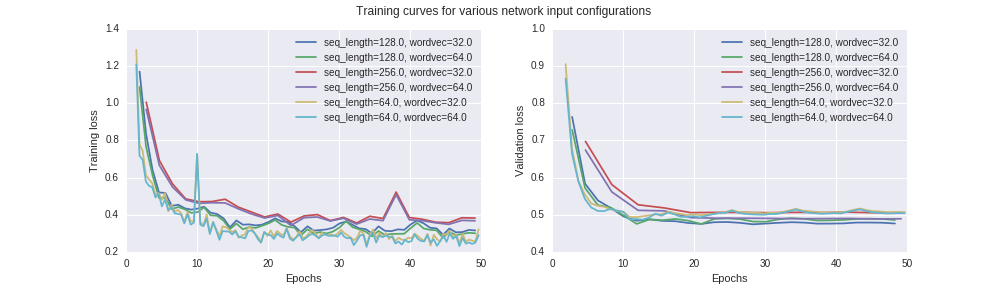
\includegraphics[width=\linewidth]{torch-rnn-input-params.png}
    \caption{torch-rnn-input-params}
    \label{fig:torch-rnn-input-params}
\end{figure}

\begin{figure}[htpb]
  \centering
  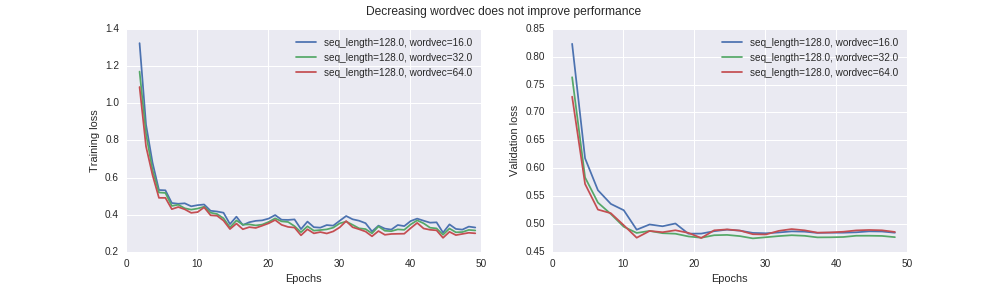
\includegraphics[width=1.0\linewidth]{torch-rnn-input-params-wordvec.png}
  \caption{torch-rnn-input-params-Wordvec}
  \label{fig:torch-rnn-input-params-wordvec}
\end{figure}

Sensitivity to network inputs: \texttt{seq\_length} and \texttt{wordvec}
\begin{itemize}
    \item Training losses are about the same across all \texttt{wordvec}s
    \item Validation losses suggest that increasing \texttt{seq\_length} important for
        good performance \mynote{investigate further}
    \item \texttt{wordvec=128} overfits for all cases, the other two depend on
        \texttt{seq\_length} and vary an order of magnitude smaller than the
        performance gains from increasing \texttt{seq\_length}
\end{itemize}

\section{Results}

\mynote{Compare with \citep{Allan2005} and \citep{Brien2016}}.

\mynote{Compare on pitch/pitch class usage, note durations, meter, lengths of compositions}

\section{Accelerating model training with GPUs}

\nomenclature[z-GPU]{GPU}{Graphics Processing Unit}

\mynote{Show speedup when training with multi-GPU, selling point is how fast the model trains}

\section{Other applications}

Scoring things as ``Bach-like'', model for expectation by using the probability.
